% !TeX root = ../main.tex

\chapter{神经网络}
\label{chap:NN}

为了识别信号中的位移喷注(displaced jets)与类标准模型(SM-like)喷注以及由束流背景(BIB)产生的伪喷注,训练了一个逐喷注(per-jet)的神经网络(NN)。
该神经网络在隐藏区域(Hidden Sector)模型信号、标准模型多喷注(SM Multi-jets)以及 BIB 的混合样本上进行训练。
神经网络的输入变量为与喷注相关的低级特征,涵盖整个 ATLAS 探测器的信息,包括径迹、量能器以及 μ 子谱仪相关信息。
训练前对每个变量进行了预处理,以确保神经网络训练的最优效果。

该神经网络基于 ATLAS 喷注味标注(flavor tagging)合作组开发的 salt~\cite{ATL-PHYS-PUB-2022-027} 框架开发。
NN 的主体结构选用基于 Transformer\cite{vaswani2023attentionneed} 的图神经网络(Graphic Neural Network, GNN)。
训练采用 Pytorch\cite{paszke2019pytorchimperativestylehighperformance} 框架,
并使用 Optuna\cite{akiba2019optunanextgenerationhyperparameteroptimization} 框架进行超参数(hyperparameter)优化。
训练结果经过评估以排除过拟合现象,并在所用信号样本上相较于此前的网络性能有所提升。

训练使用的信号区域(signal region)数据集包括来自探测器的 BIB 数据(见\autoref{sec:detector_data})
和信号与标准模型多喷注(简记为 QCD)模拟数据(见\autoref{sec:MC})。
训练中使用的喷注均为 clean 喷注,其定义见\autoref{sec:jet_preselection}。
信号喷注为隐藏区域(Hidden Sector)模型中由一系列不同的$m_\Phi$、$m_s$、$c\tau$参数生成的模拟数据,
其中 $m_\Phi$ 为中介粒子质量,$m_s$ 为 LLP 的质量,$c\tau$ 为 LLP 衰变长度。
训练阶段仅使用事件编号为奇数的信号事件,偶数编号的事件则用于后续分析流程,以避免因数据重叠而引发的偏差,确保最终结果的客观性和可信度。
对于 QCD 喷注,训练样本来自 JZ2W、JZ3W 和 JZ4W 样本,
这些样本覆盖了 \pt 范围为 60 GeV 至 800 GeV 的双喷注(dijet)事件,叠加的 pileup 喷注将该范围的下界扩展至 40 GeV。
BIB 喷注训练样本选取触发 HLT CalRatio 触发器但未通过 HLT BIB 抑制算法的事件。
随后通过 $\Delta R$ 匹配离线喷注与触发喷注,匹配成功并满足公共选择条件的喷注被标记为 BIB 喷注。

为了进行补充训练以及计算本分析中使用的机器学习方法的系统不确定性,需要在数据和 MC 模拟中定义一个控制区域(control region)。
控制区域中所选样本具有统一的筛选条件(见\autoref{cpm:CR_jet_selection}),以确保喷注来源于相同的产生机制,并覆盖相同的运动学范围。
控制区域数据包括探测器数据和 QCD 模拟数据。

信号区域上定义的主数据集总计有 2.09M jets,其中 766k jets 属于信号集、660k jets 属于 QCD 集、660k jets 属于 BIB 集。
控制区域上定义的补充数据集总计有 449k jets,其中 223k jets 属于 MC 模拟、226k jets 属于探测器。

由于信号与背景喷注可通过 ATLAS 探测器的各个子系统加以刻画,因此神经网络也应当充分利用来自各子探测器的信息。
NN 输入变量的概述如下(详见\autoref{cpm:NN_variables}):
\begin{itemize}
    \item 位于喷注轴线 $\Delta R < 0.2$ 范围内的径迹的空间位置、动量、碰撞参数(impact parameter)和径迹拟合质量参量(quality variables);
    \item 与喷注相关联的拓扑集团(topo-clusters) 的动量、时间信息和空间位置;
    \item 喷注在电磁量能器与强子量能器各层的能量沉积比例;
    \item 位于喷注 $\Delta \phi < 0.2$ 范围内的μ子段(muon segment)的空间与时间信息;
    \item 喷注本身的动量与空间位置。
\end{itemize}

训练前对所有输入变量(设为$x$)进行归一化预处理
\begin{equation}
    x' = \frac{x-\mu}{\sigma}
\end{equation}
其中$\mu$为该变量分布的均值、$\sigma$为标准差,
使得处理后该变量分布的均值为0、标准差为1,以加快训练收敛速度。
预处理完成后,喷注输入至神经网络,网络输出对应于信号、QCD 与 BIB 的预测权值。


\section{网络结构}
\begin{figure}[ht]
    \centering
    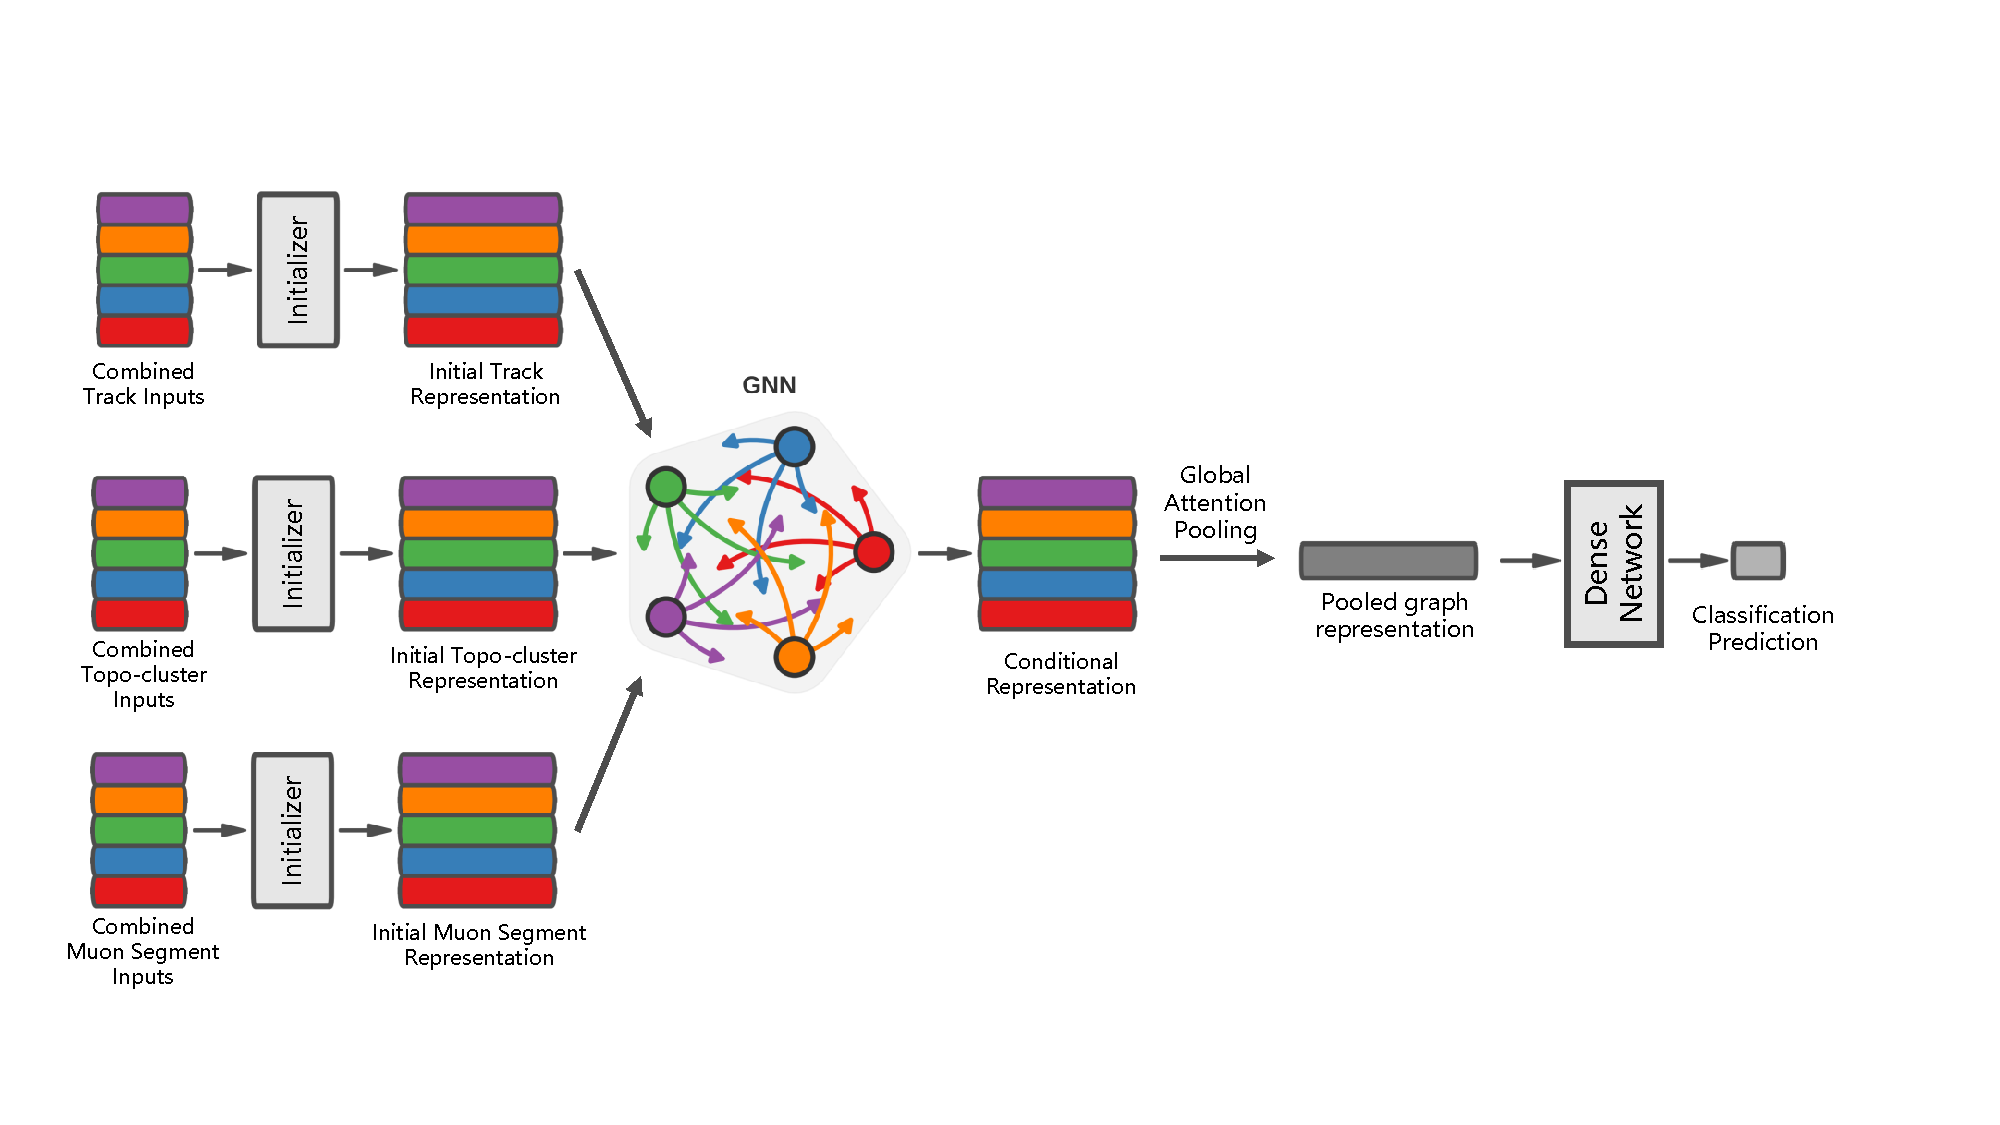
\includegraphics[width=\textwidth]{CalRatio_GNN_Architecture.pdf}
    \caption{GNN 网络结构示意图}
    \label{fig:CalRatio_GNN_Architecture}
\end{figure}

逐喷注神经网络的结构如\autoref{fig:CalRatio_GNN_Architecture} 所示。
多个来自径迹、量能器和 μ 子谱仪的输入变量被分别输入至用于初始化的子网络(initializer)中,得到维度相同的向量表示。
每个向量表示作为全连接图神经网络的节点,根据节点之间的相关性计算注意力权重作为边值。
然后利用 Transformer 机制更新节点表示得到下一层 GNN,最后一层 GNN 的所有节点经过池化(pooling)得到单向量特征表示。
将该特征表示传入全连接层分类器,得到最终分类的预测值。

基于 Transformer 的 GNN 兼顾了节点自身的特征提取(通过自注意力机制)和节点间的相关性(通过注意力边值),
获得了更好的特征提取与表示能力,得到了相较于卷积神经网络(CNN)\cite{ATLAS:2022zhj} 更好的性能(见\autoref{fig:ROC})。


\subsection{初始化网络}
初始化网络的作用类似于大语言模型(LLM)中的嵌入层(embedding layer),
用来将输入变量映射为高维向量表示。

\begin{figure}[ht]
    \centering
    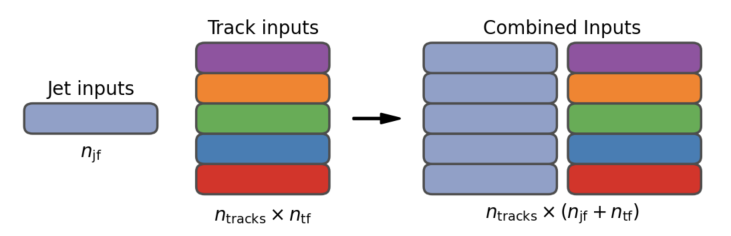
\includegraphics[width=0.7\textwidth]{input_concatenate.png}
    \caption{输入变量拼接示意图}
    \label{fig:input_concatenate}
\end{figure}

以径迹为例,由于模型的输入包括喷注和径迹两个层级的输入变量,它们各自的特征维度不同($n_\text{jf}=3, n_\text{tf}=10$),
而一个喷注中将选取 20 条径迹作为输入($n_\text{tracks}=20$),所以需要将喷注输入变量复制后与每个径迹输入变量拼接,
得到一个$n_\text{tracks} \times (n_\text{jf} + n_\text{tf})$维度的联合输入(combined input),如\autoref{fig:input_concatenate} 所示。
对于拓扑集团(topo-cluster)和 μ 子段的拼接处理同理,它们的数量与特征维度为
$n_\text{\topos} = 30, n_\text{tcf}=12, n_\text{muon-segments}=30, n_\text{msf}=6$。

初始化网络为几个全连接层组成的多层感知器(Multi-layer perceptron, MLP),负责得到各个输入变量初始化后的高维向量表示。
每一类输入变量对应一个初始化网络,它们有着不同的输入层维度,对应不同类别输入的特征维度,
但具有相同的隐藏层(hidden layer)维度和输出层维度。
初始化网络具有相同的输出维度是为了在后续的 GNN 中将不同类别的输入变量视为同质的(homogeneous)。


\subsection{图神经网络}
初始化后的特征表示被输入至基于 Transformer 的图神经网络(GNN)中,GNN 由多个 GNN 层组成。
每一层 GNN 由两个子网络组成,分别为多头注意力(multi-head attention)网络和多层感知器(MLP)。
其中多头注意力网络用于提取节点间的相关性,构成图结构的边值;多层感知器用于更新节点的特征表示。

多头注意力网络通过在多个子空间并行执行缩放点积注意力,使模型能够从不同角度捕获序列依赖关系。
在 Transformer 中,输入特征矩阵 ${X}\in\mathbb{R}^{n\times d_{\mathrm{model}}}$
($n$为 GNN 节点数,$d_{\mathrm{model}}$ 为初始化网络的输出维数)
分别与三组可训练的投影矩阵相乘,生成查询(Query)、键(Key)和值(Value)矩阵
\begin{align}
    {Q} & = {X}\,W^Q, \quad W^Q \in\mathbb{R}^{d_{\mathrm{model}}\times d_k}, \\
    {K} & = {X}\,W^K, \quad W^K \in\mathbb{R}^{d_{\mathrm{model}}\times d_k}, \\
    {V} & = {X}\,W^V, \quad W^V \in\mathbb{R}^{d_{\mathrm{model}}\times d_v}.
\end{align}
其中${Q}$表示“我在寻找什么”,用于与所有键做相似度匹配;
${K}$作为每个位置的“标签”,与查询计算注意力权重;
${V}$携带实际输出信息,根据注意力分数完成加权聚合。
节点 $i$ 的查询向量 ${Q}_i$ 与节点 $j$ 的键向量 ${K}_j$ 的点积 ${Q}_i \cdot {K}_j$
为图结构里节点 $j$ 指向节点 $i$的边值,代表了第 $i$ 个查询与第 $j$ 个键之间的相似度,点积越大表示它们之间的相关性越强。
矩阵形式的缩放点积注意力(scaled dot-product attention)为
\begin{align}
    \mathrm{Attention}({Q},{K},{V})
    = \mathrm{softmax} \Bigl(\frac{{Q}\,{K}^\top}{\sqrt{d_k}}\Bigr)\,{V}
    \cite{vaswani2023attentionneed}
\end{align}
其中,除以 $\sqrt{d_k}$ 用于缓解高维点积过大带来的梯度不稳定问题。

在缩放点积注意力的基础上引入多头注意力机制,使得 NN 可以在多个子空间并行执行注意力计算,以捕获不同类型的依赖关系。
令头数为 $h$,并为每一头准备独立的线性投影
\[
    Q_i = QW_i^Q,\quad
    K_i = KW_i^K,\quad
    V_i = VW_i^V,\quad
    W_i^Q,W_i^K,W_i^V\in\mathbb{R}^{d_{\text{model}}\times d_k},
    \quad i=1,\dots,h
\]
在第 $i$ 个子空间上执行注意力计算
\begin{align}
    \mathrm{head}_i & = \mathrm{Attention}(Q_i, K_i, V_i)
\end{align}
将所有头的输出拼接后,再通过线性变换映射回原始维度
\begin{align}
    \mathrm{MultiHead}(Q,K,V)
     & = \mathrm{Concat}\bigl(\mathrm{head}_1,\dots,\mathrm{head}_h\bigr)\,W^O,
    \quad W^O\in\mathbb{R}^{hd_v\times d_{\text{model}}}
    \cite{uvadlc2025}.
\end{align}

在得到每个节点的多头注意力后,GNN 通过多层感知器(MLP)对节点进行更新。
MLP 由两个线性变换和一个激活函数(ReLU)组成,以“线性变换-激活函数-线性变换”的顺序排列。
GNN 更新后的节点值为
\begin{equation}
    h'_i = \mathrm{MLP}\bigl(\mathrm{MultiHead}(Q,K,V)\bigr)_i + h_i,
    \quad i=1,\dots,n
\end{equation}

重复上述 GNN 加 MLP 的操作多次,得到最终的节点表示。


\subsection{池化层}
GNN 的输出为 $n$ 个节点的向量表示,池化层用于将 GNN 的输出节点表示通过加权和的方式转换为单个向量表示。
池化层由一个线性层和一个 softmax 层组成,
线性层的输入维度为 GNN 的输出向量维度,输出维度为 1,用于产生每个节点的初始权重$a_i$
\begin{equation}
    a_i = \mathrm{Linear}(h'_i), \quad i=1,\dots,n,
    \quad a_i\in\mathbb{R}^1
\end{equation}
每个节点的初始权值经过 softmax 层后,得到每个节点的权值 $w_i$
\begin{equation}
    w_i = \frac{\exp(a_i)}{\sum_{j=1}^n \exp(a_j)}, \quad i=1,\dots,n
\end{equation}
池化层的输出 $p$ 为所有节点的加权和
\begin{equation}
    p = \sum_{i=1}^n w_i h'_i,
    \quad p\in\mathbb{R}^{d_{\text{model}}}
\end{equation}


\subsection{分类器}
池化层的输出 $p$ 被输入至分类器中,分类器为具有三个隐藏层的 MLP,输出维度为 3,
经过 softmax 处理后对应于信号、QCD 和 BIB 的预测权值。


\section{训练方法}
\begin{figure}[ht]
    \centering
    \subfloat[signal]{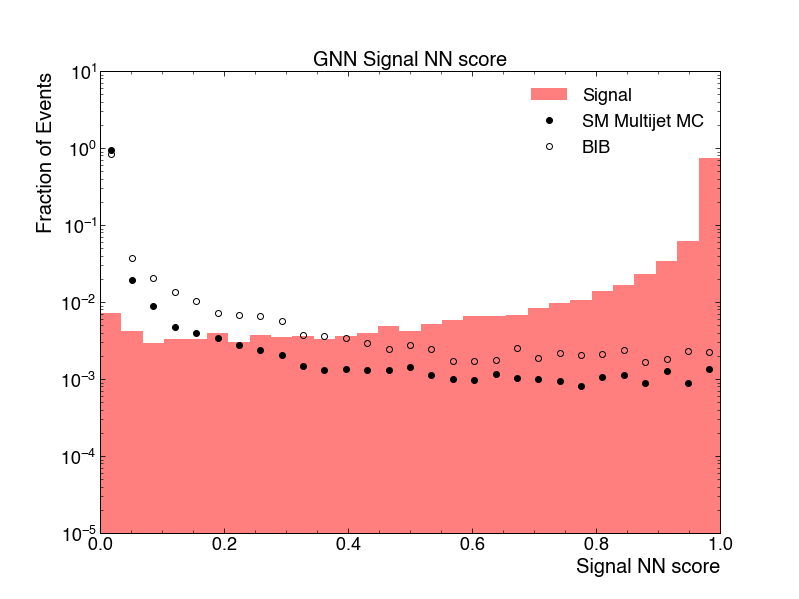
\includegraphics[width=0.33\textwidth]{GNN_sig_before.png}}
    \hfill
    \subfloat[QCD]{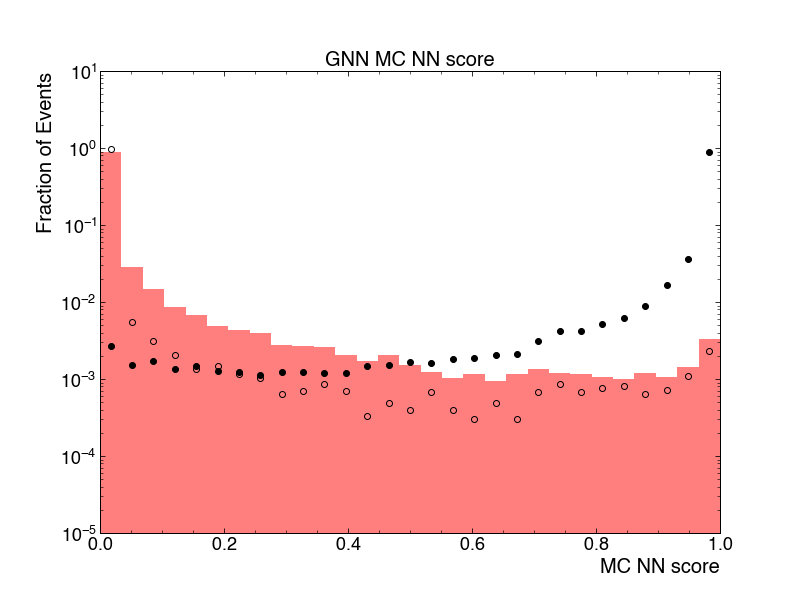
\includegraphics[width=0.33\textwidth]{GNN_QCD_before.png}}
    \hfill
    \subfloat[BIB]{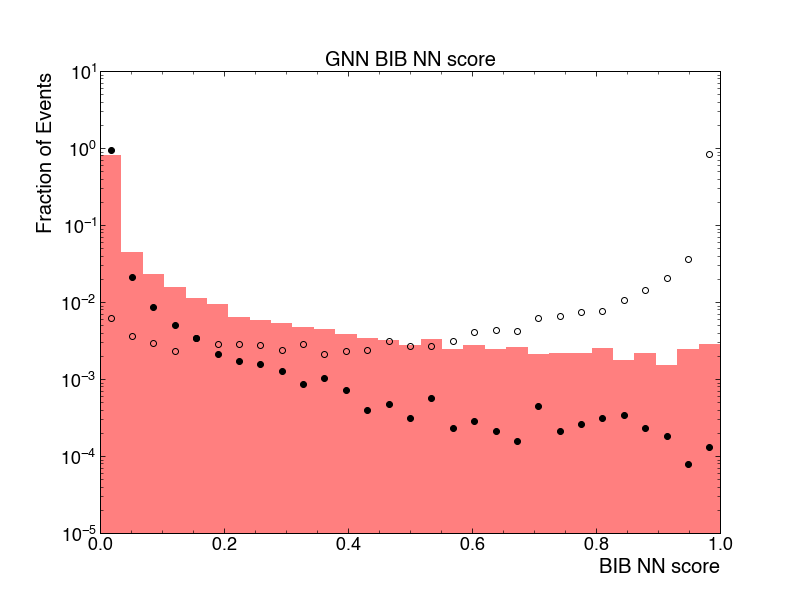
\includegraphics[width=0.33\textwidth]{GNN_BIB_before.png}}
    \caption{GNN 在信号区域的预测分数分布}
    \label{fig:GNN_before}
\end{figure}

\begin{figure}[ht]
    \centering
    \subfloat[CNN]{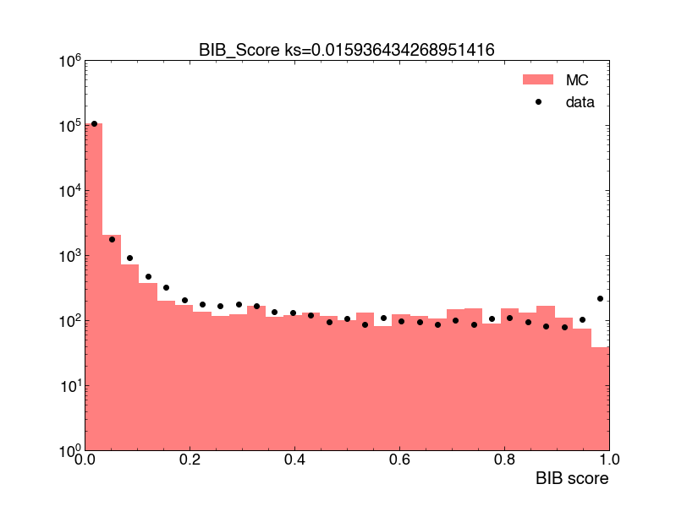
\includegraphics[width=0.49\textwidth]{CNN_CR.png}}
    \hfill
    \subfloat[GNN]{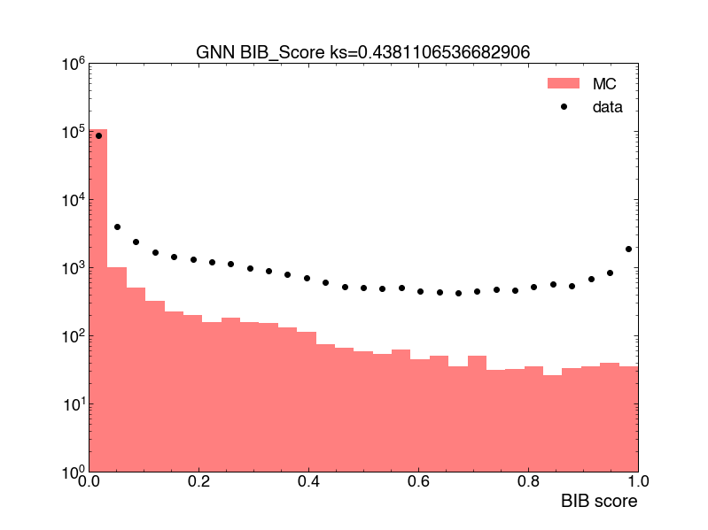
\includegraphics[width=0.49\textwidth]{GNN_CR_before.png}}
    \caption{NN 在控制区域的 BIB 预测分数分布}
    \label{fig:CR_BIB_before}
\end{figure}

NN 在信号区域的预测分数分布如\autoref{fig:GNN_before} 所示,
可以看到信号、QCD 和 BIB 的预测分数分布均呈现出良好的分离。
NN 在控制区域的 BIB 预测分数分布如\autoref{fig:CR_BIB_before} 所示,
与文献\cite{ATLAS:2022zhj} 中加入对抗网络的 CNN 结果相比,
GNN 的 BIB 预测分数分布在真实数据(data)和模拟数据(MC)上呈现较大差别。
所以需要引入控制区域的数据和新的训练方法来改善这一问题。

\begin{figure}[ht]
    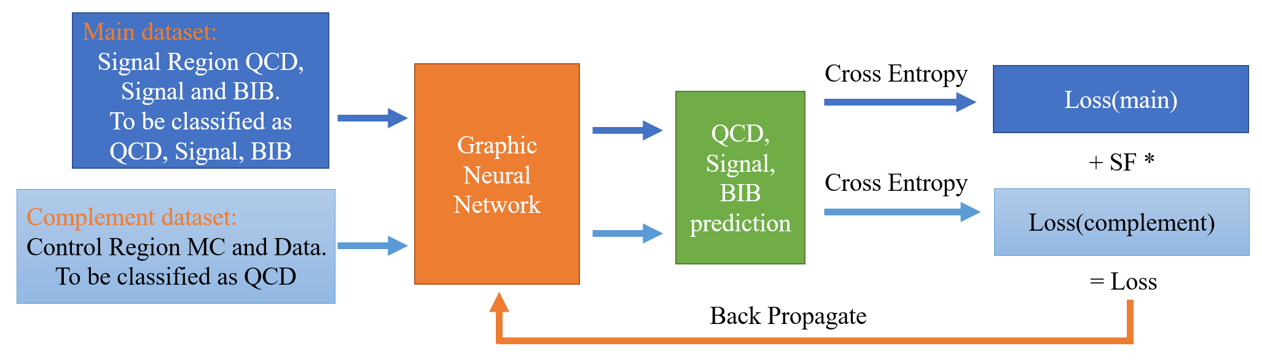
\includegraphics[width=\textwidth]{GNN_complement_workflow.png}
    \caption{GNN 补充训练流程示意图}
    \label{fig:GNN_complement_workflow}
\end{figure}

% 文献\cite{ATLAS:2022zhj} 提出的训练方法为:在神经网络输出后添加一个对抗网络(adversarial network),
% 该网络用于在控制区中学习区分模拟喷注与真实数据喷注的特征,并将此反馈至主网络以抑制数据与 MC 的不一致性。
由于控制区域的喷注样本均为 QCD 喷注,想要让神经网络无法区分模拟数据与真实数据,
可以直接将控制区域的 QCD 喷注与信号区域的 QCD 喷注混合在一起进行训练。
为了更好的灵活性,将控制区域数据的影响用一个随训练迭代次数变化的权重 $\lambda$ 控制,
对应的损失函数为
\begin{equation}
    \text{loss} = \text{loss}(\text{signal region}) + \lambda \cdot \text{loss}(\text{control region})
\end{equation}
随迭代步数变化的权重因子为
\begin{equation}
    \lambda(x) = \begin{cases}
        0,                                    & x < a        \\
        \lambda_{\max} \cdot \frac{x-a}{b-a}, & a \leq x < b \\
        \lambda_{\max},                       & x \geq b
    \end{cases}
\end{equation}
其中$x \in [0, 1]$为当前迭代步数占预期总迭代步数的比例,$a$ 决定什么时候控制区域数据开始起作用,
$b$ 决定什么时候控制区域数据的影响力达到最大值,$\lambda_{\max}$ 决定控制区域数据的最大影响力。
$a$、$b$ 和 $\lambda_{\max}$ 为自由选取的超参数,仅需要满足$a<b$。
加入控制区域数据集的 GNN 补充训练流程示意图如\autoref{fig:GNN_complement_workflow} 所示。


\section{训练结果}
\begin{figure}[ht]
    \centering
    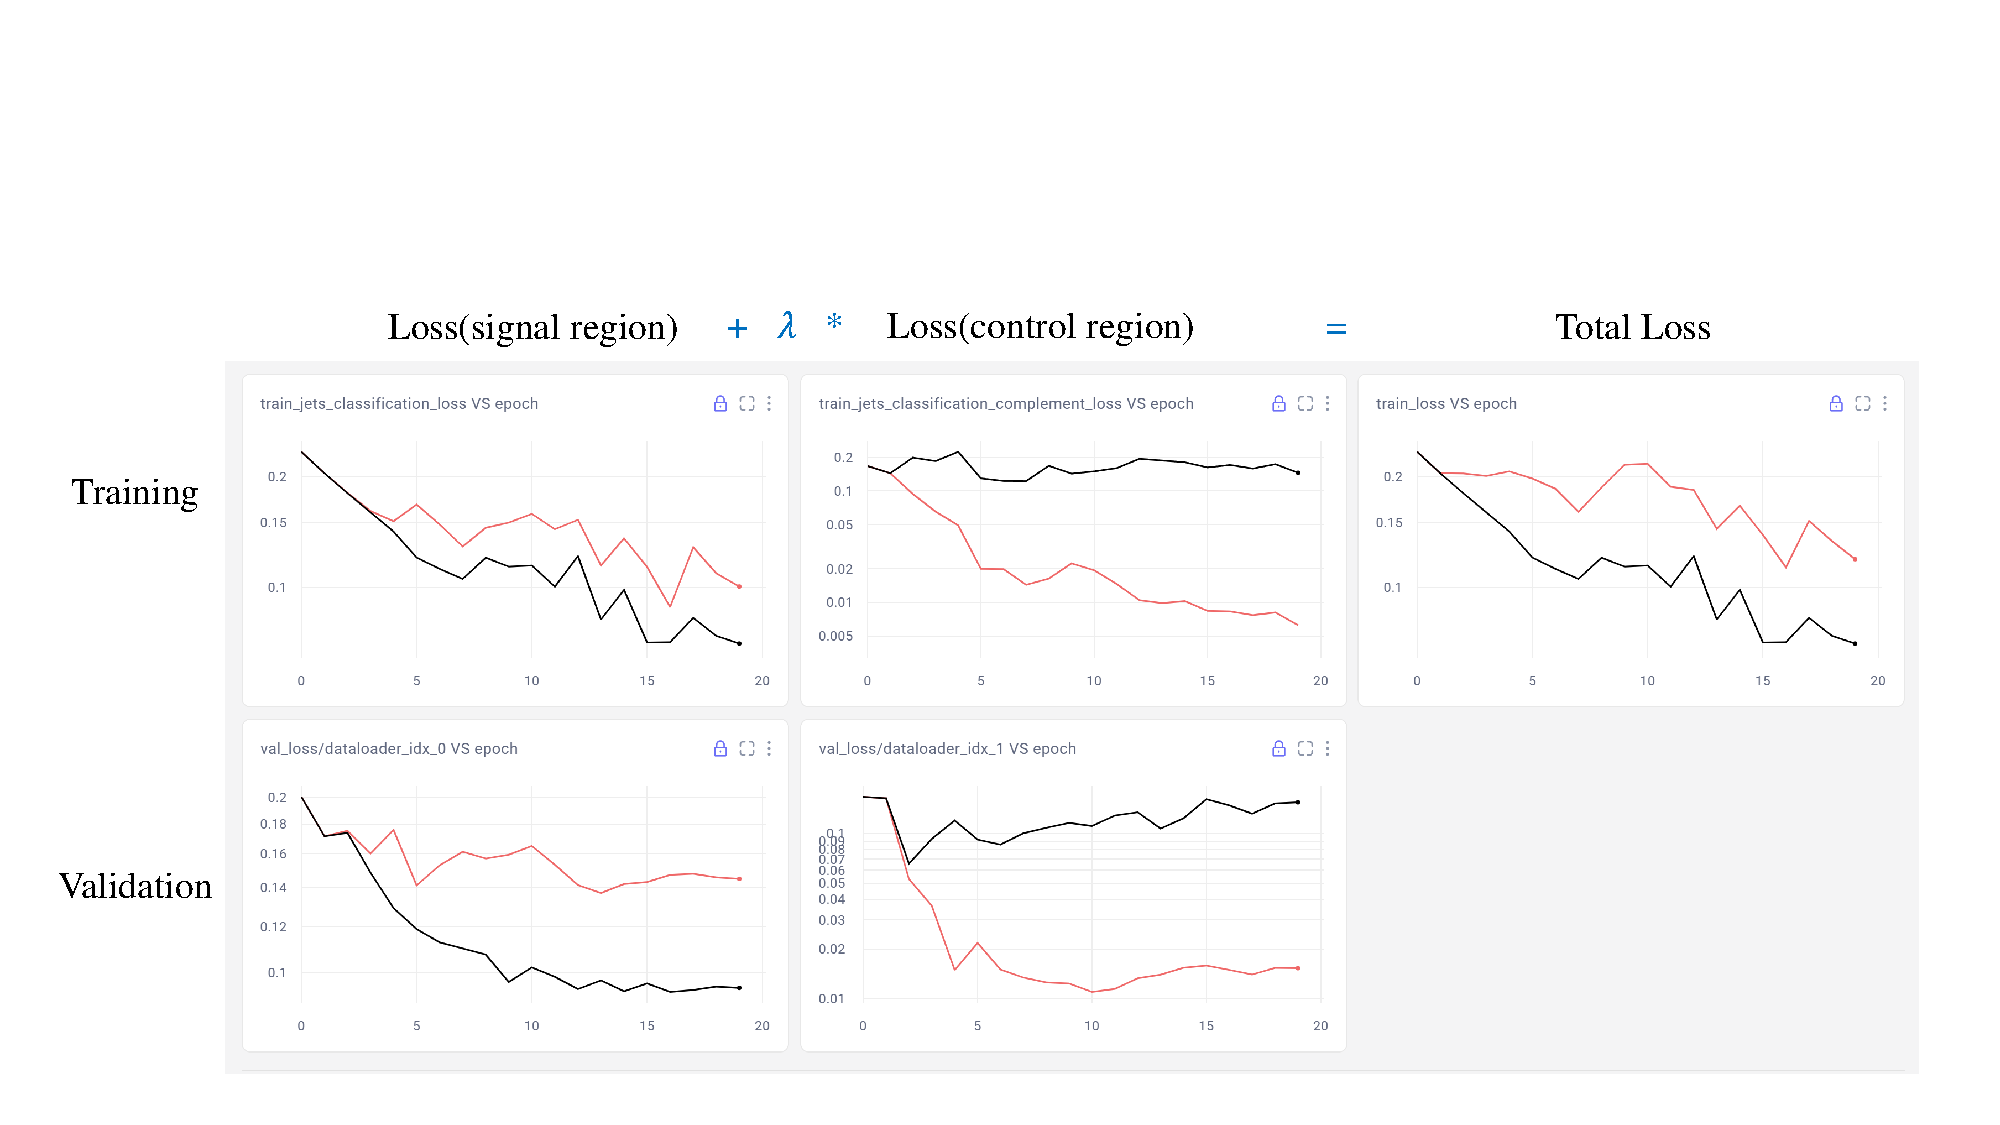
\includegraphics[width=\textwidth]{GNN_loss.pdf}
    \caption{在训练集和验证集上的损失函数}
    \label{fig:GNN_loss}
    \figurenote{注:黑线未加入控制区域数据($\lambda_{\max}=0$)的贡献,红线加入控制区域数据。}
\end{figure}

\begin{figure}[ht]
    \centering
    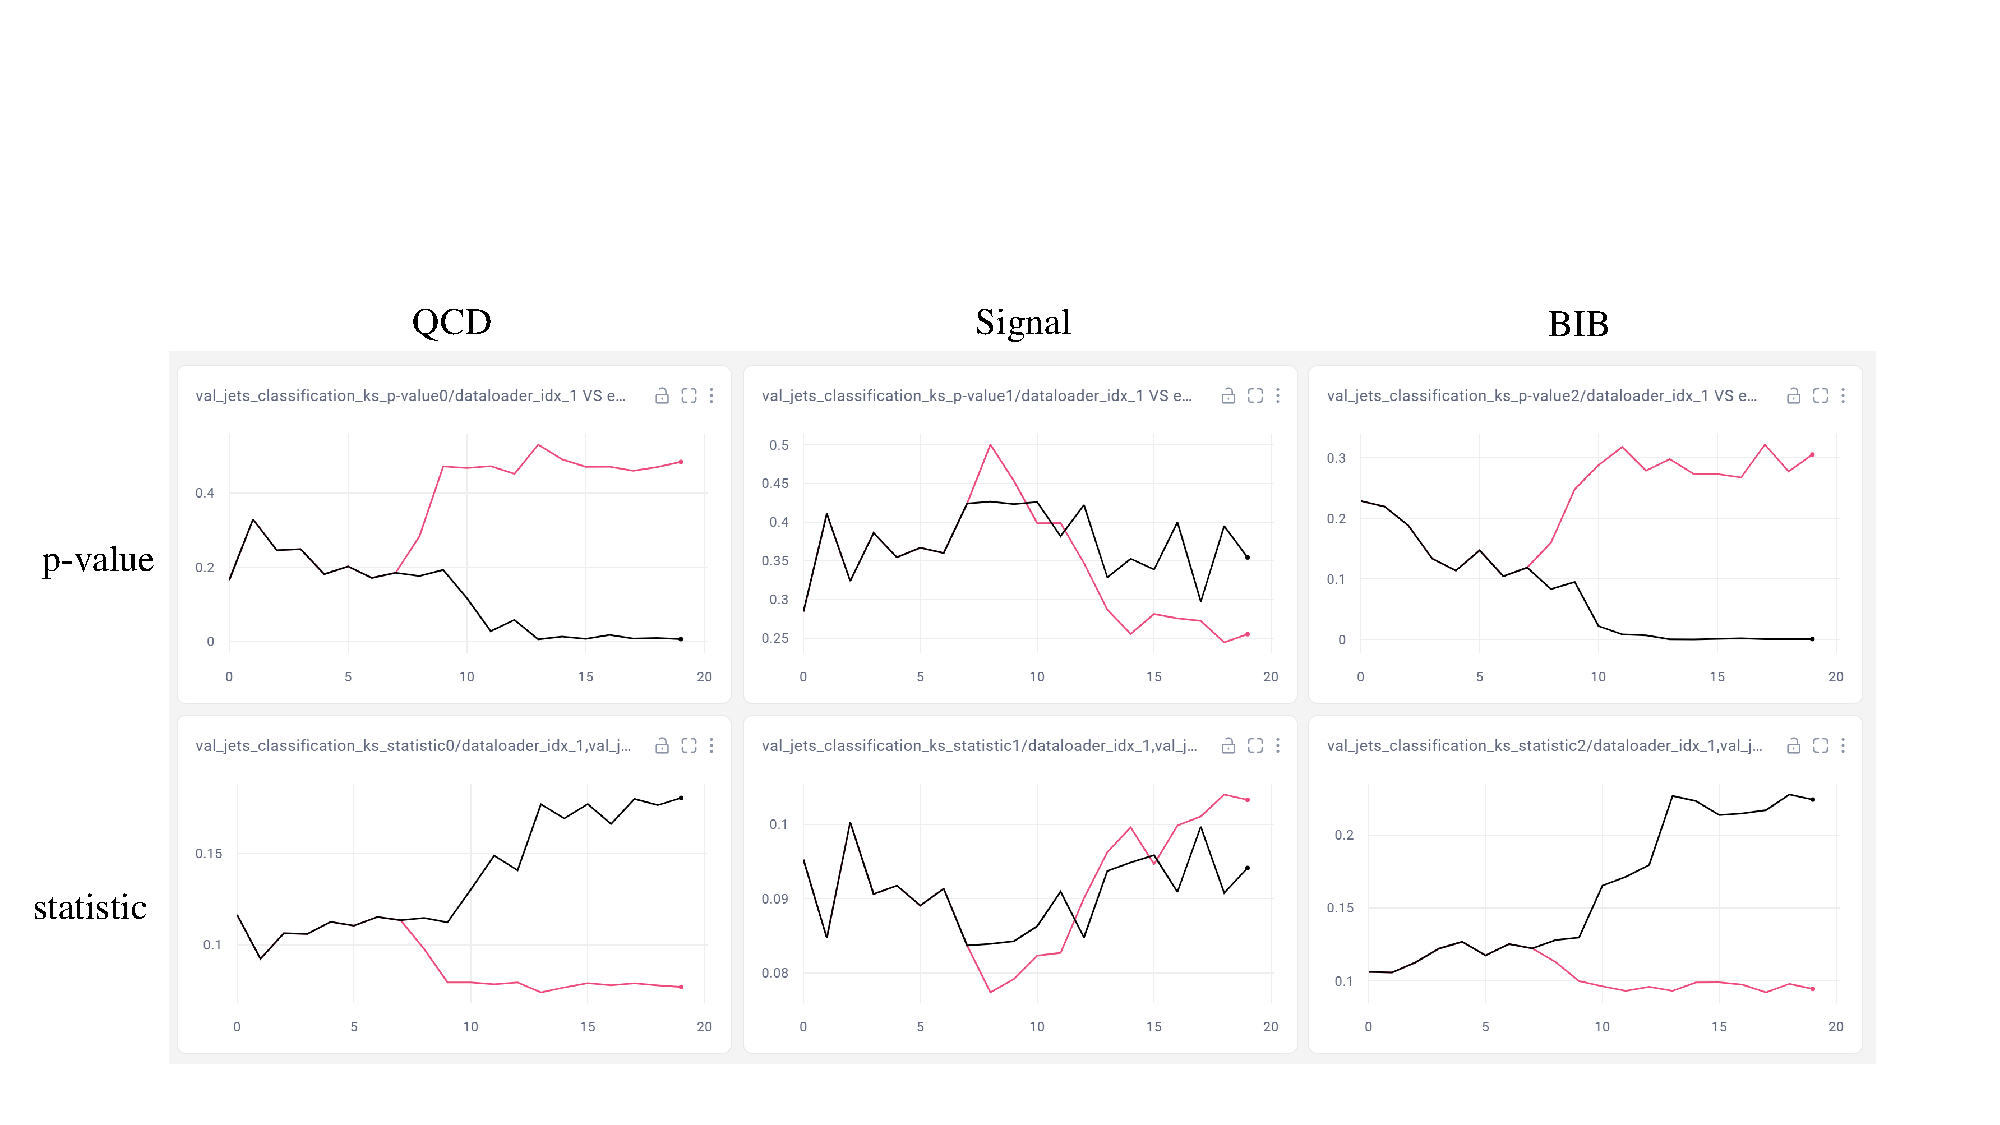
\includegraphics[width=\textwidth]{GNN_ks.pdf}
    \caption{在控制区域验证集上的 KS 检验结果}
    \label{fig:GNN_ks}
    \figurenote{注:黑线未加入控制区域数据($\lambda_{\max}=0$)的贡献,红线加入控制区域数据。}
\end{figure}

训练过程中损失函数的变化如\autoref{fig:GNN_loss} 所示,
可以看到加入控制区域数据后,控制区域的损失函数有明显下降,但同时影响信号区域的损失函数。
用 KS 检验(Kolmogorov-Smirnov test)评估真实数据与模拟数据的分布差异,
其统计量$D$(KS statistic)为两者累计分布函数(CDF)的最大差异
\begin{equation}
    D = \max\limits_{x} |F_1(x) - F_2(x)|
\end{equation}
统计量的值越小表示两者分布越接近。
$p$值($p$-value)为 $D$ 统计量对应的概率,
$p$ 值越大表示两者分布越接近。
KS 检验的结果如\autoref{fig:GNN_ks} 所示,
可以看到加入控制区域数据后,在 QCD 类别与 BIB 类别的 KS 检验结果均有明显改善,
说明 GNN 在控制区域的性能有了显著提升。

为对数坐标与非对数坐标下的控制区域 BIB 预测分数分布,
可以看到加入控制区域数据参与训练后,GNN 的 BIB 预测分数分布的一致性有了明显改善。

\begin{figure}[ht]
    \centering
    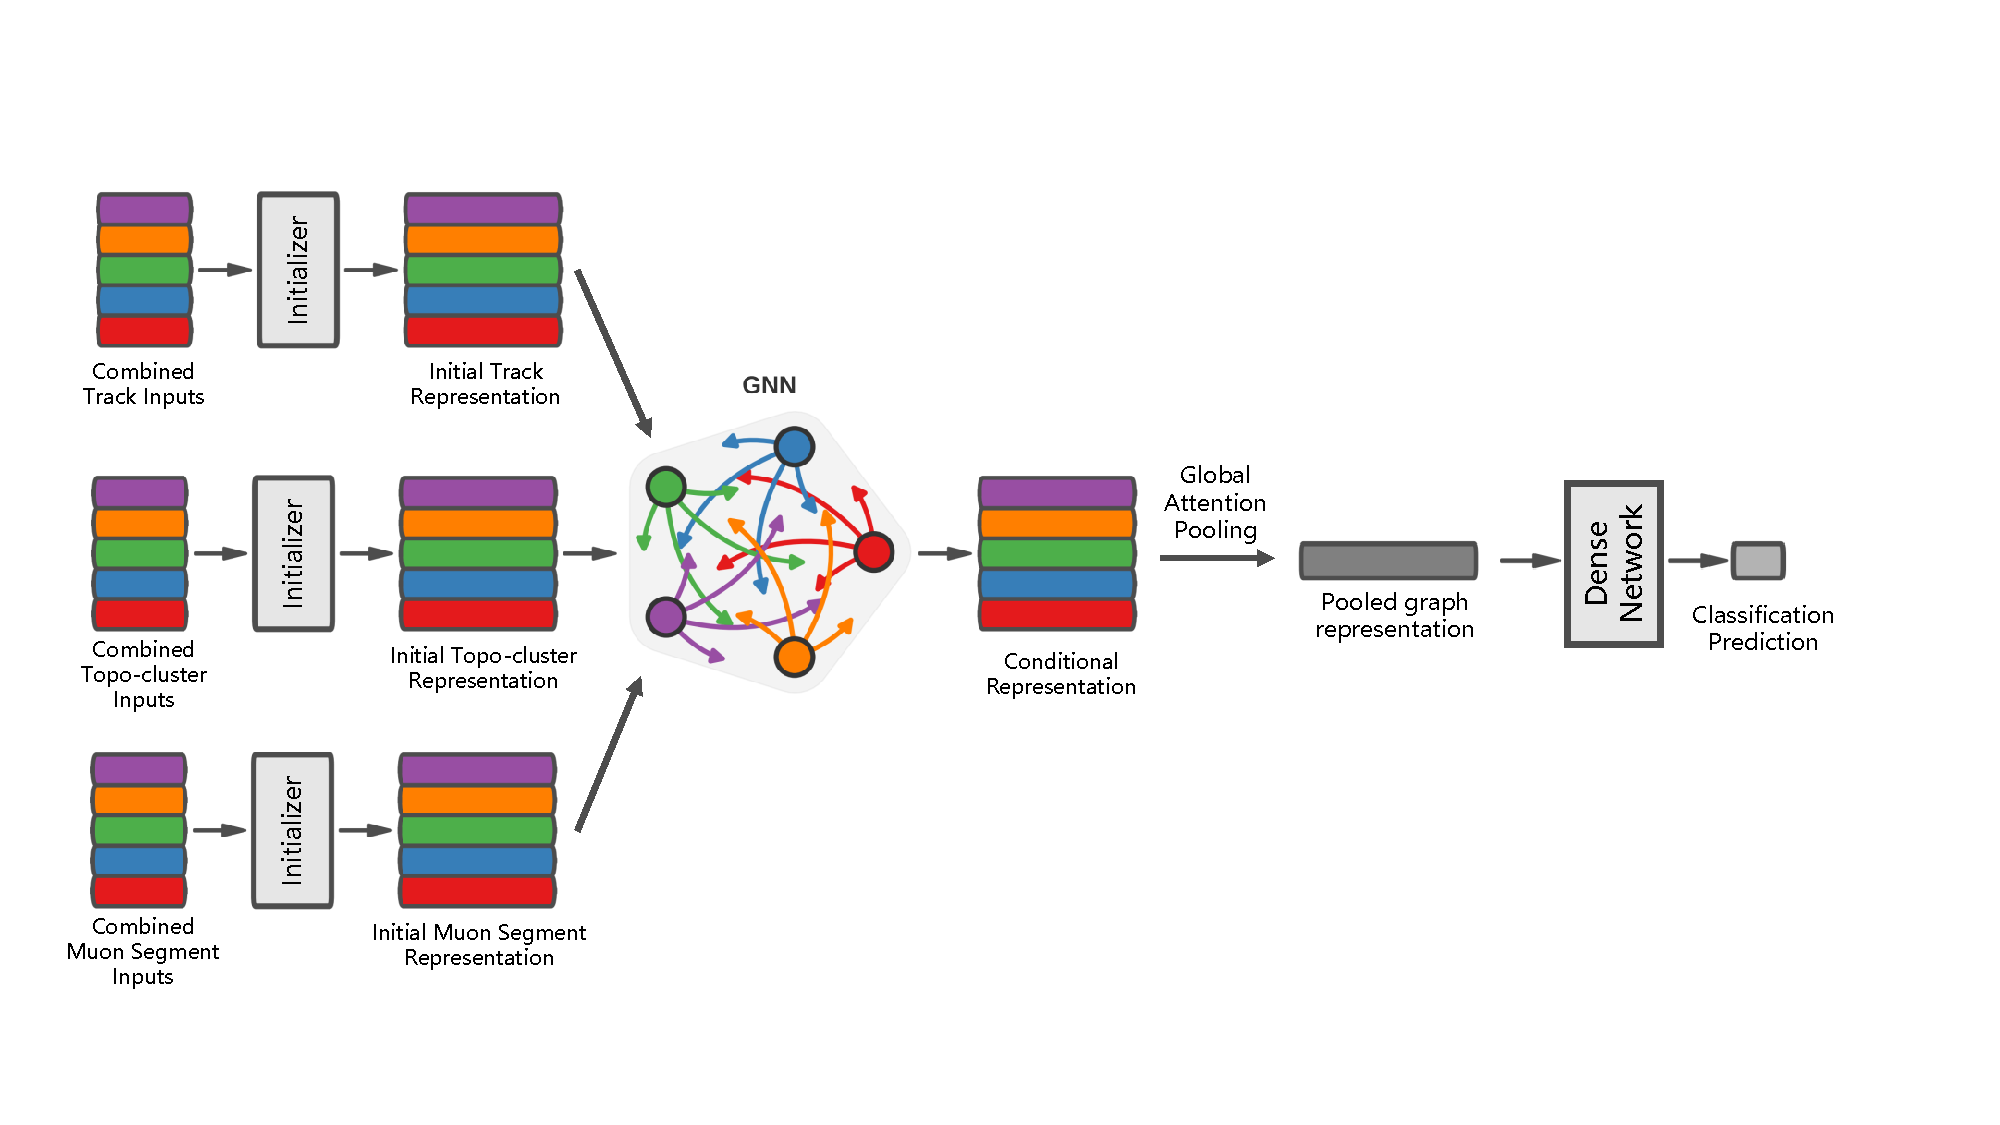
\includegraphics[width=\textwidth]{CalRatio_GNN_Architecture.pdf}
    \caption{ROC}
    \label{fig:ROC}
\end{figure}

加入控制区域数据集前后的 GNN 和文献\cite{ATLAS:2022zhj} 中的 CNN 的 ROC 曲线如\autoref{fig:ROC} 所示,
可以看到加入控制区域数据在一定程度上影响了 GNN 在信号区域的性能,
但相较于文献\cite{ATLAS:2022zhj} 中的 CNN,GNN 的性能仍然有明显提升。
